\section{Auswertung}
\label{sec:Auswertung}

\subsection{Fehlerrechnung}

Für die Fehlerfortpflanzung bei Gleichungen mit $N$ fehlerbehafteten Größen
wird jeweils die Formel zur Gaußschen Fehlerfortpflanzung

\begin{equation*}
  \sigma = \sqrt{\sum_{i=1}^{N}\biggl(\frac{\partial f(x_{\g{i}})}{\partial x_{\g{i}}}
  \sigma_{\g{i}}\biggr)^2}
\end{equation*}
mit der jeweiligen Funktion $f(x_{\g{i}})$, den Messgrößen $x_{\g{i}}$ und den
zugehörigen Fehlern $\sigma_i$ verwendet.

Zur Berechnung des arithmetischen Mittels von $N$ Messwerten wird jeweils die Formel

\begin{equation*}
  \bar{x} = \frac{1}{N}\sum_{i=1}^{N}x_{\g{i}}
\end{equation*}
benutzt.

\newpage

Die Standardabweichung des Mittelwerts wird jeweils mit der Gleichung

\begin{equation*}
  \bar{\sigma} = \sqrt{\frac{1}{N-1}\sum_{i=1}^{N}(x_{\g{i}} - \bar{x})^2}
\end{equation*}
berechnet.

\subsection{Amplitudenmodulierte Schwingung mit Ringmodulator}

Mit Hilfe der Schaltung aus Abbildung \ref{fig:expab} wird eine Amplitudenmodulierte Schwingung erzeugt.
Diese so entstandene Schwebung ist in Abbildung \ref{fig:amplModOszi} zu sehen.

\begin{figure}[h]
  \centering
  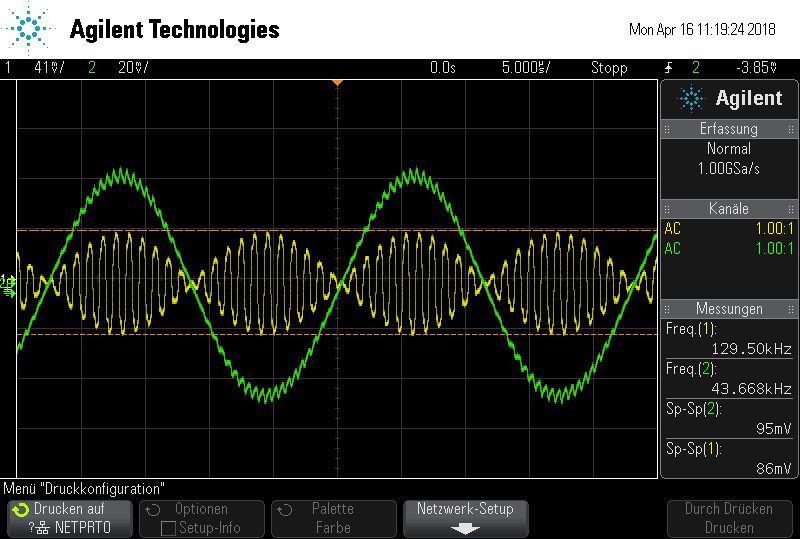
\includegraphics[width=.9\textwidth]{Oszi_Pics/amplModRing.png}
  \caption{Amplitudenmodulierte Schwingung(gelb) und Modulationsschwingung(grün) erzeugt mit Ringmodulator.}
  \label{fig:amplModOszi}
\end{figure}

Die mit dem Oszilloskop außerdem ausgemessenen Werte für die Frequenzen $f$ und Amplituden $U_\text{peak to peak}$ der Modulationsspannung $M$ und der Trägerspannung $T$ sind:

\begin{align*}
  f_\text{M} &= \SI{43.8(5)}{\kilo\hertz} & U_\text{M, ptp} &= \SI{95(1)}{\milli\volt}\\
  f_\text{T} &= \SI{970(1)}{\kilo\hertz} & U_\text{T, ptp} &= \SI{540(1)}{\milli\volt}.
\end{align*}

Die mit dem Frequenzspektrometer aufgenommenen Werte sind in den Bildern \ref{fig:b1}, \ref{fig:b2} und \ref{fig:b3} zu sehen.

\begin{figure}[h]
  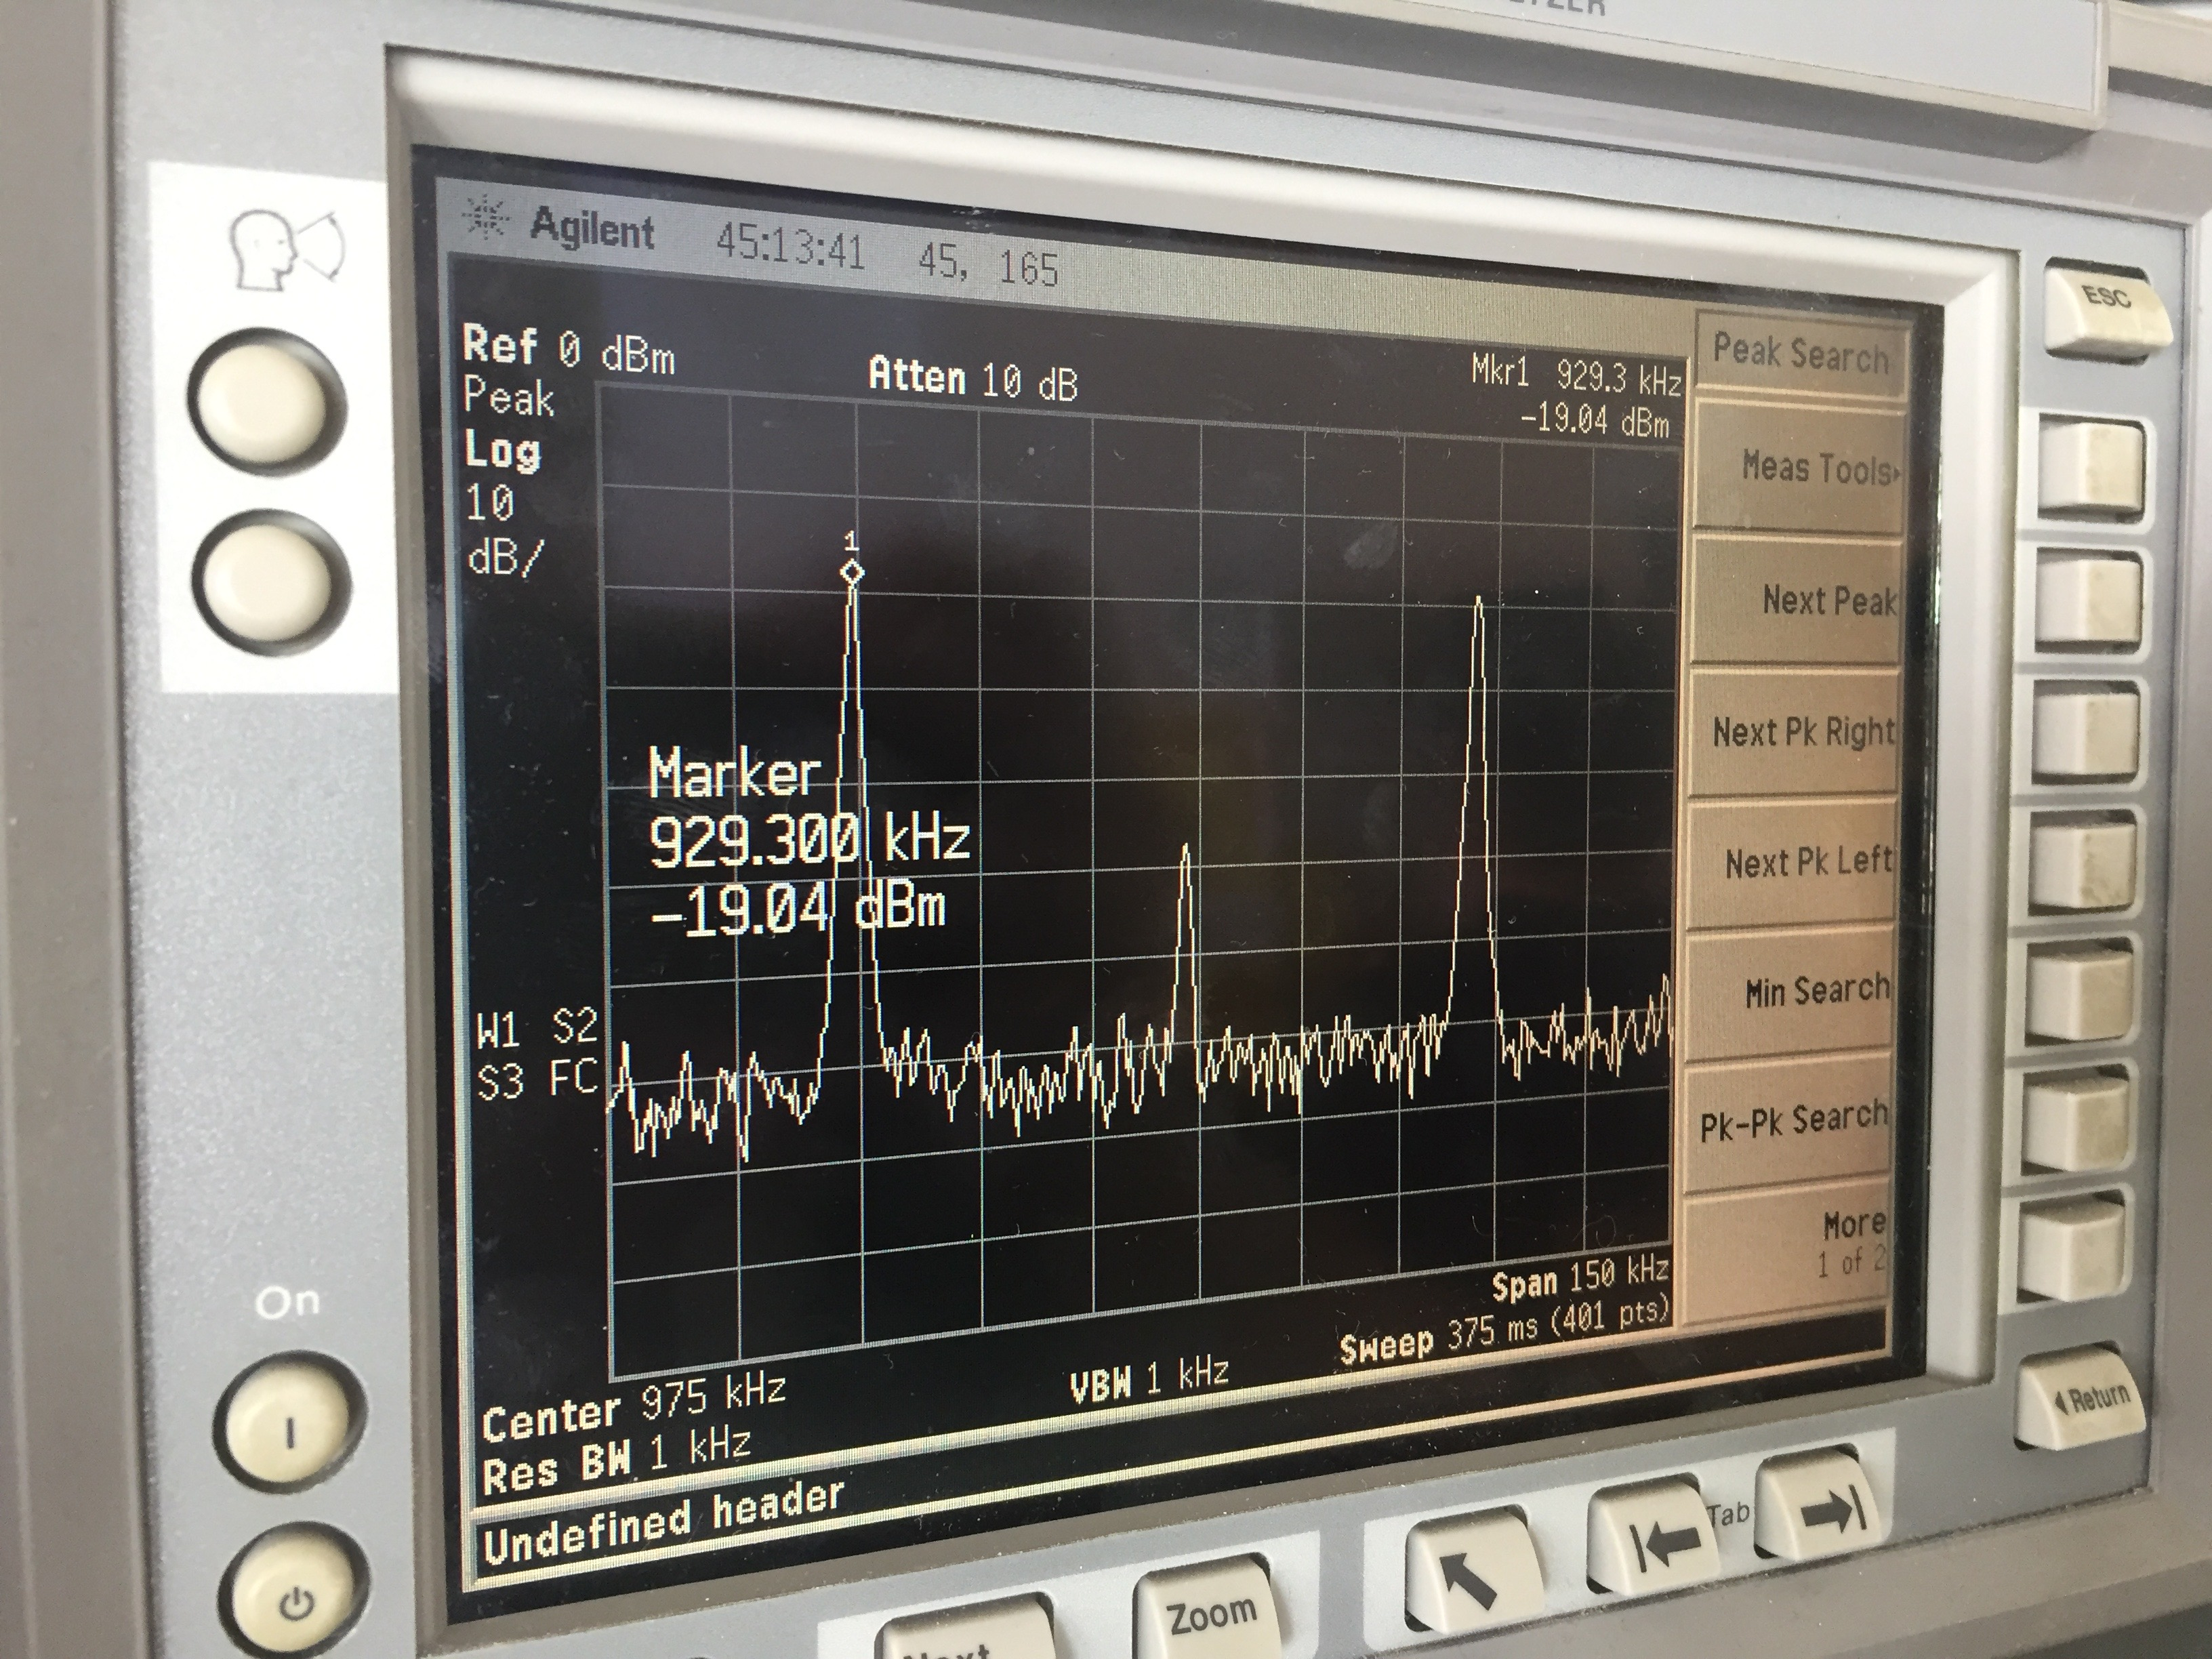
\includegraphics[width=.9\textwidth]{Spektrum_Pics/b1.jpg}
  \caption{Spektrum der mit dem Ringmodulator amplitudenmodulierten Schwingung mit Markierung vom Peak $f_\text{T} - f_\text{M}$}
  \label{fig:b1}
\end{figure}


Die aus dem Frequenzspektrum abgelesenen Frequenzen und Leistungspegel für die drei größten Peaks sind:
\begin{align*}
  f_1 &= \SI{929.3}{\kilo\hertz} & f_2 &= \SI{973.1}{\kilo\hertz} & f_3 &= \SI{1016.6}{\kilo\hertz}.\\
  L_{\text{P}, 1} &= \SI{-19.04}{dBm} & L_{\text{P}, 2} &= \SI{-47.6}{dBm} & L_{\text{P}, 3} &= \SI{-19.02}{dBm}
\end{align*}
Die Abweichungen zu den erwarteten Werten betragen:
\begin{align*}
  \frac{|(f_\text{T} - f_\text{M}) - f_1|}{f_\text{T} - f_\text{M}} &= \SI{0.3(1)}{\percent}\\
  \frac{|f_\text{T} - f_2|}{f_\text{T}} &= \SI{0.3(1)}{\percent}\\
  \frac{|(f_\text{T} + f_\text{M}) - f_3|}{f_\text{T} + f_\text{M}} &= \SI{0.3(1)}{\percent}.
\end{align*}

\subsection{Amplitudenmodulierte Schwingung mit Diode}
\label{sec:amplModDiode}

Nach Schaltung aus Abbildung \ref{fig:expc} wird hier der allgemeine Fall der Amplitudenodulation mit einer Diode gezeigt.

\begin{figure}[h]
  \centering
  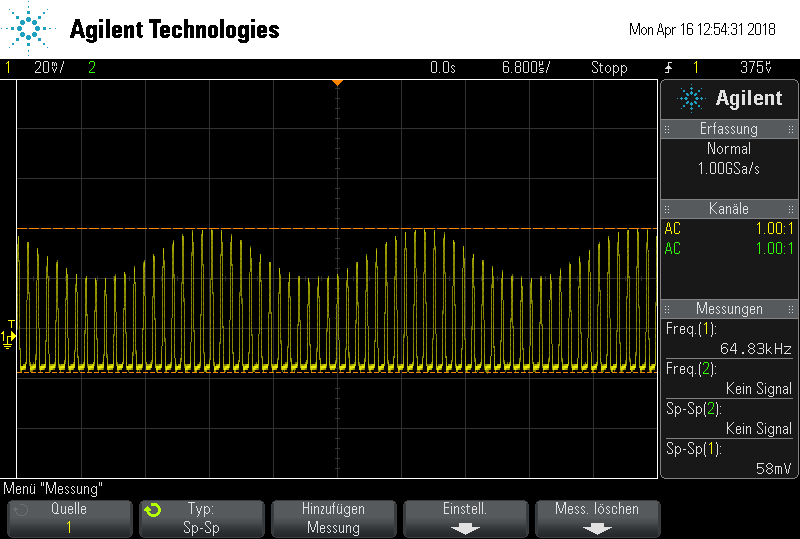
\includegraphics[width=.9\textwidth]{Oszi_Pics/amplModDiode.png}
  \caption{Amplitudenmodulierte Schwingung erzeugt mit einer Diode.}
  \label{fig:amplModDiode}
\end{figure}

Die so entstandene Schwebung ist in Abbildung \ref{fig:amplModDiode} zu sehen.
Außerdem wurden folgende Kennzahlen der modulierten Spannung ausgemessenen:
die Spannungsdifferenz von der Nulllinie im Oszilloskop bis zum höchsten Wert $U_\text{max}$, die Differenz zwischen der höchsten und der niedrigsten Amplitude $U_\text{diff}$ sowie die Spannungsdifferenz von der Nulllinie bis zur unteren Kante also der Fehler der Diode $U_\text{fehler}$.
Diese Werte betragen:
\begin{align*}
  U_\text{max} &= \SI{43(1)}{\milli\volt} & U_\text{diff} &= \SI{20(1)}{\milli\volt}  & U_\text{fehler} &= \SI{14(1)}{\milli\volt}
\end{align*}
Aus Bild \ref{fig:amplmodskizze} wird die Formel
\begin{align}
  m &= \frac{U_\text{max}}{U_\text{max} - \frac{U_\text{diff}}{2}} - 1\\
  \intertext{hergeleitet.}
  \intertext{Das ergibt für den Modulationsgrad:}
  m &= \num{0.30(2)}.
\end{align}

Nun wird der Modulationsgrad aus der Frequenzspektrumsmessung abgelesenen.
\begin{figure}[h]
  \centering
  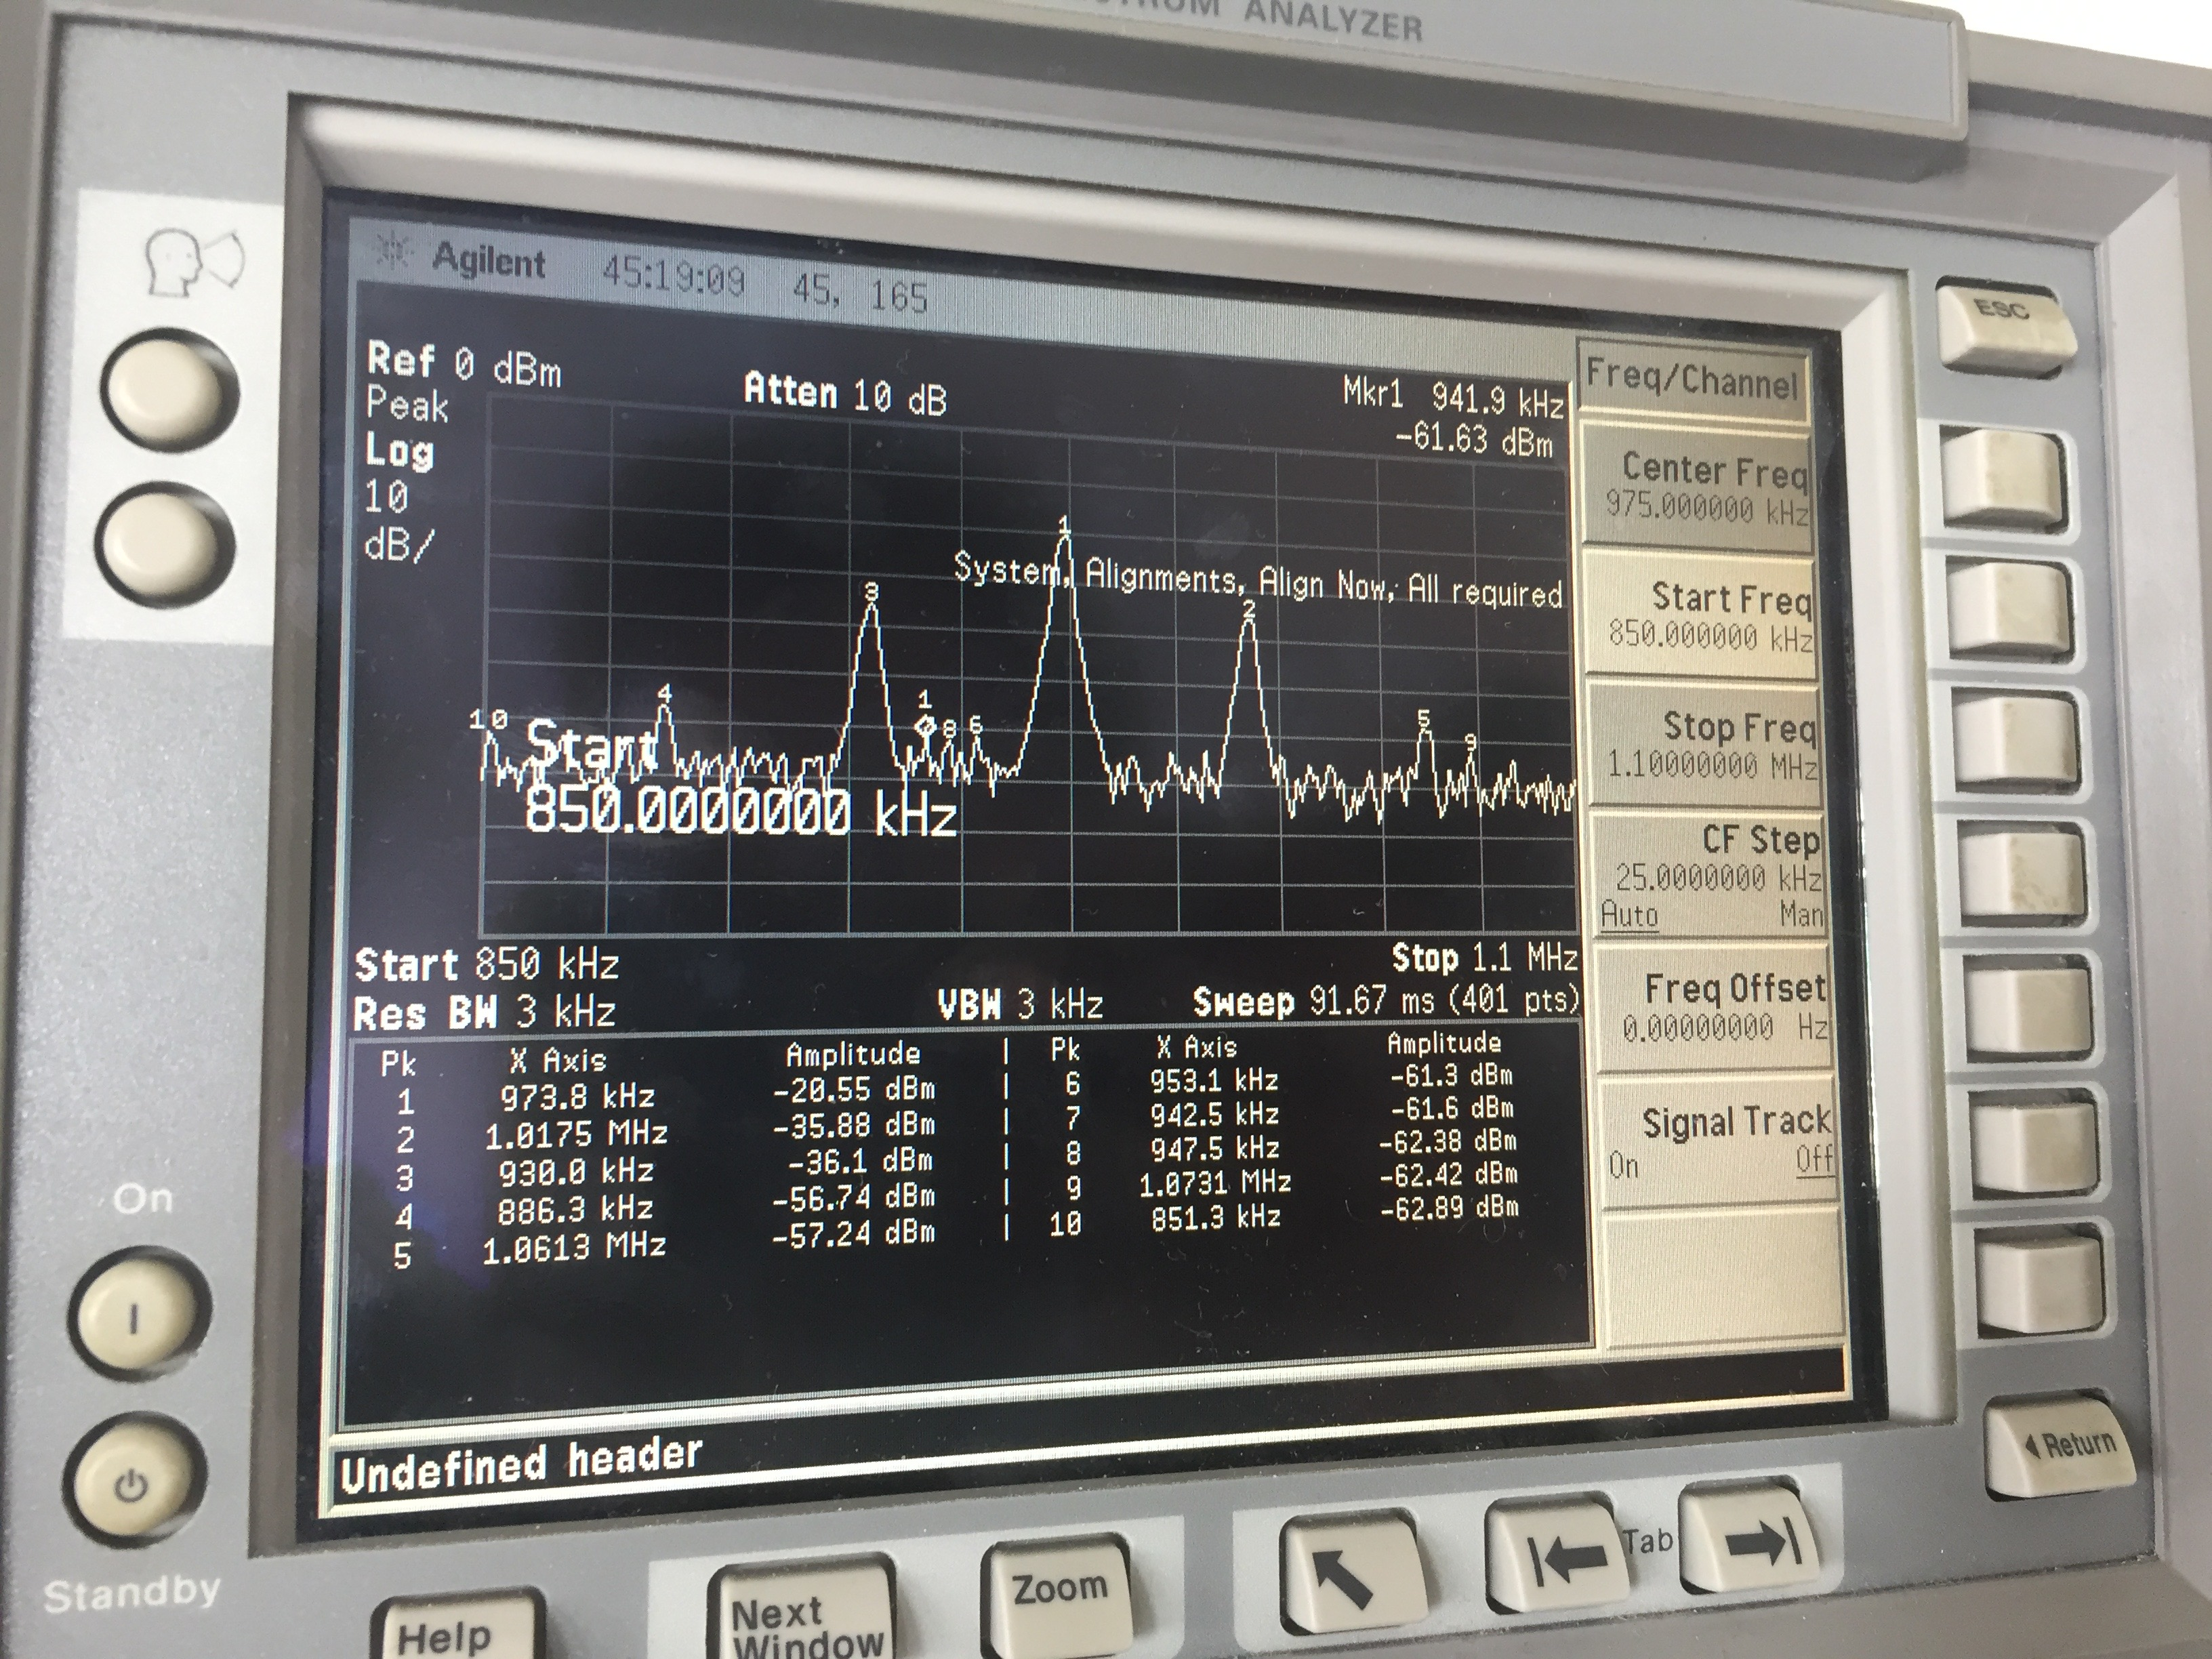
\includegraphics[width=.9\textwidth]{Spektrum_Pics/c.jpg}
  \caption{Spektrum der mit der Diode amplitudenmodulierten Schwingung mit einer Peaktable.}
  \label{fig:c}
\end{figure}
Das Bild mit dem Spektrum der Frequenzen ist in Abbildung \ref{fig:c} zu sehen.
Dabei werden die drei höchsten Peaks den Frequenzen $f_\text{T} - f_\text{M}$, $f_\text{T}$ und $f_\text{T} + f_\text{M}$ zugeordnet.
Die Peaktable zeigt die Werte für die Leistungspegel $L_\text{P}$:
\begin{align*}
  L_\text{P, links} &= \SI{-36.1(1)}{dBm} & L_\text{P, mitte} &= \SI{-20.55(10)}{dBm} & L_\text{P, rechts} &= \SI{-35.88(10)}{dBm}.
\end{align*}
Diese Werte werden nun mit Gleichung \eqref{eqn:dBmTomW} aus \cite{leistungspegel} umgerechnet in Werte für die Leistung der Frequenzen.
\begin{align}
  P(\si{\milli\watt}) =
   10^{\frac{L_\text{P}(\si{dBm})}{10}} \SI{1}{\milli\watt} \label{eqn:dBmTomW}
\end{align}

Diese betragen:
\begin{align*}
  P_\text{links} &= \SI{0.245(6)}{\micro\watt} & P_\text{mitte} &= \SI{8.81(2)}{\micro\watt} & P_\text{rechts} &= \SI{0.258(6)}{\micro\watt}.
\end{align*}
Diese Werte für die Leistung werden mit
\begin{align}
  U &= \sqrt{P R}
\end{align}
in die entsprechenden Spannungen umgerechnet. Dabei ist der Widerstand $R$ konstant.
Aus Bild \ref{fig:freqspektrum} wird nun die Formel zur Bestimmung des Modulationsgrad aus einem Frequenzspektrum hergeleitet:
\begin{align*}
  m &= \frac{2 U_\text{lr}}{U_\text{mitte}}.
\end{align*}

Hierbei ist $U_\text{lr}$ der Mittelwert des linken und des rechten Peaks der drei Peaks mit der höchsten Leistung.
So ergibt sich für $m$:
\begin{align*}
  m &= \num{0.338(5)}.
\end{align*}

\subsection{Frequenzmodulierte Schwingung}

Es wurde eine frequenzmodulierte Schwingung erzeugt mit den Frequenzen:
\begin{align*}
  f_\text{M} = \SI{211.5(4)}{\kilo\hertz} \quad\text{und}\quad f_\text{T} = \SI{973(2)}{\kilo\hertz}.
\end{align*}
\begin{figure}[h]
  \centering
  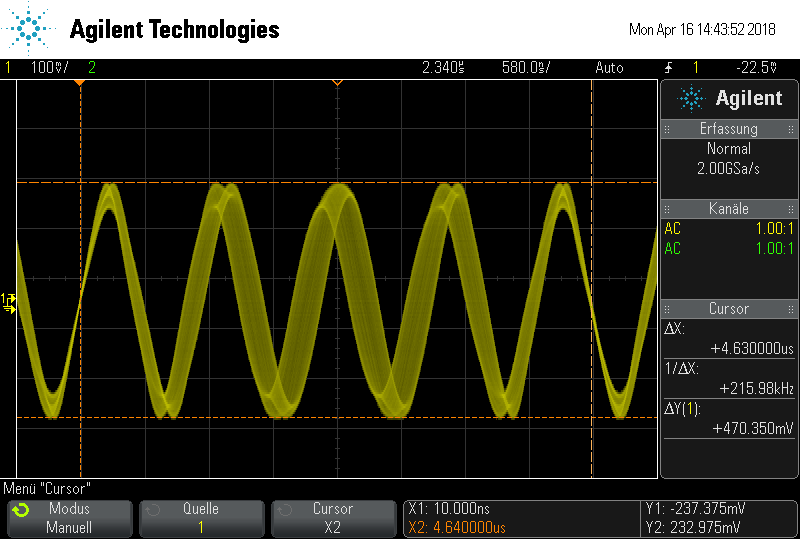
\includegraphics[width=.9\textwidth]{Oszi_Pics/freqModRing.png}
  \caption{Oszilloskopbild der frequenzmodulierten Schwingung.}
  \label{fig:freqModRing}
\end{figure}
\begin{figure}[h]
  \centering
  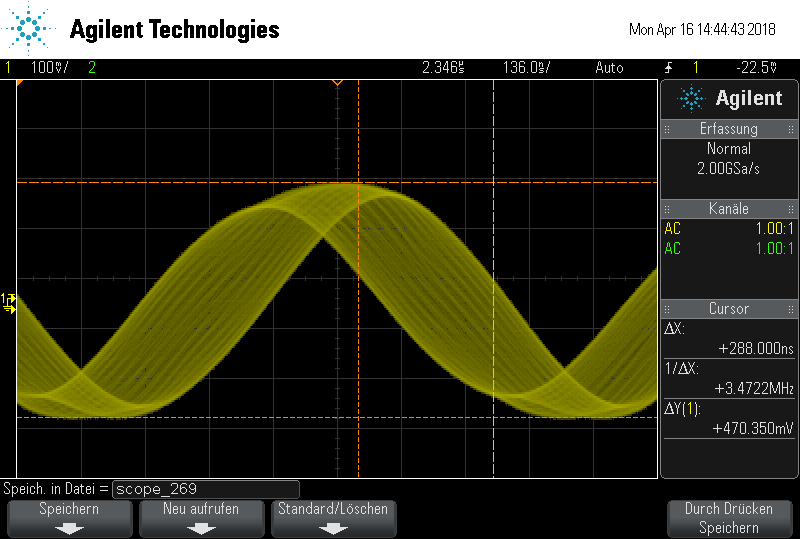
\includegraphics[width=.9\textwidth]{Oszi_Pics/freqModZoom.png}
  \caption{Vergrößertes Oszilloskopbild der frequenzmodulierten Schwingung.}
  \label{fig:freqModZoom}
\end{figure}
In Abbildung \ref{fig:freqModRing} ist die in X-Richtung verschmierte Sinuskurve der nach Schaltung \ref{fig:freqmodschaltung} frequenzmodulierten Schwingung zu sehen. Außerdem ist in Abbildung \ref{fig:freqModZoom} eine vergrößerte Version der Schwingung zu sehen. Daraus wird die Zeitdifferenz bei maximaler Frequenzvariation abgelesenen:
\begin{align*}
  t_2 - t_1 &= \SI{288(5)}{\nano\second}.\\
\intertext{Damit ergibt sich eingesetzt in Formel \eqref{eqn:mfuerfreqmod} für den Modulationsgrad}
  m &= \num{0.097(2)}.
\end{align*}

Der Modulationsgrad wird erneut auch mit dem Frequenzspektrum bestimmt. Das Bild des Spektrometers ist in Abbildung \ref{fig:freqModSpek} zu sehen.
\begin{figure}[h]
  \centering
  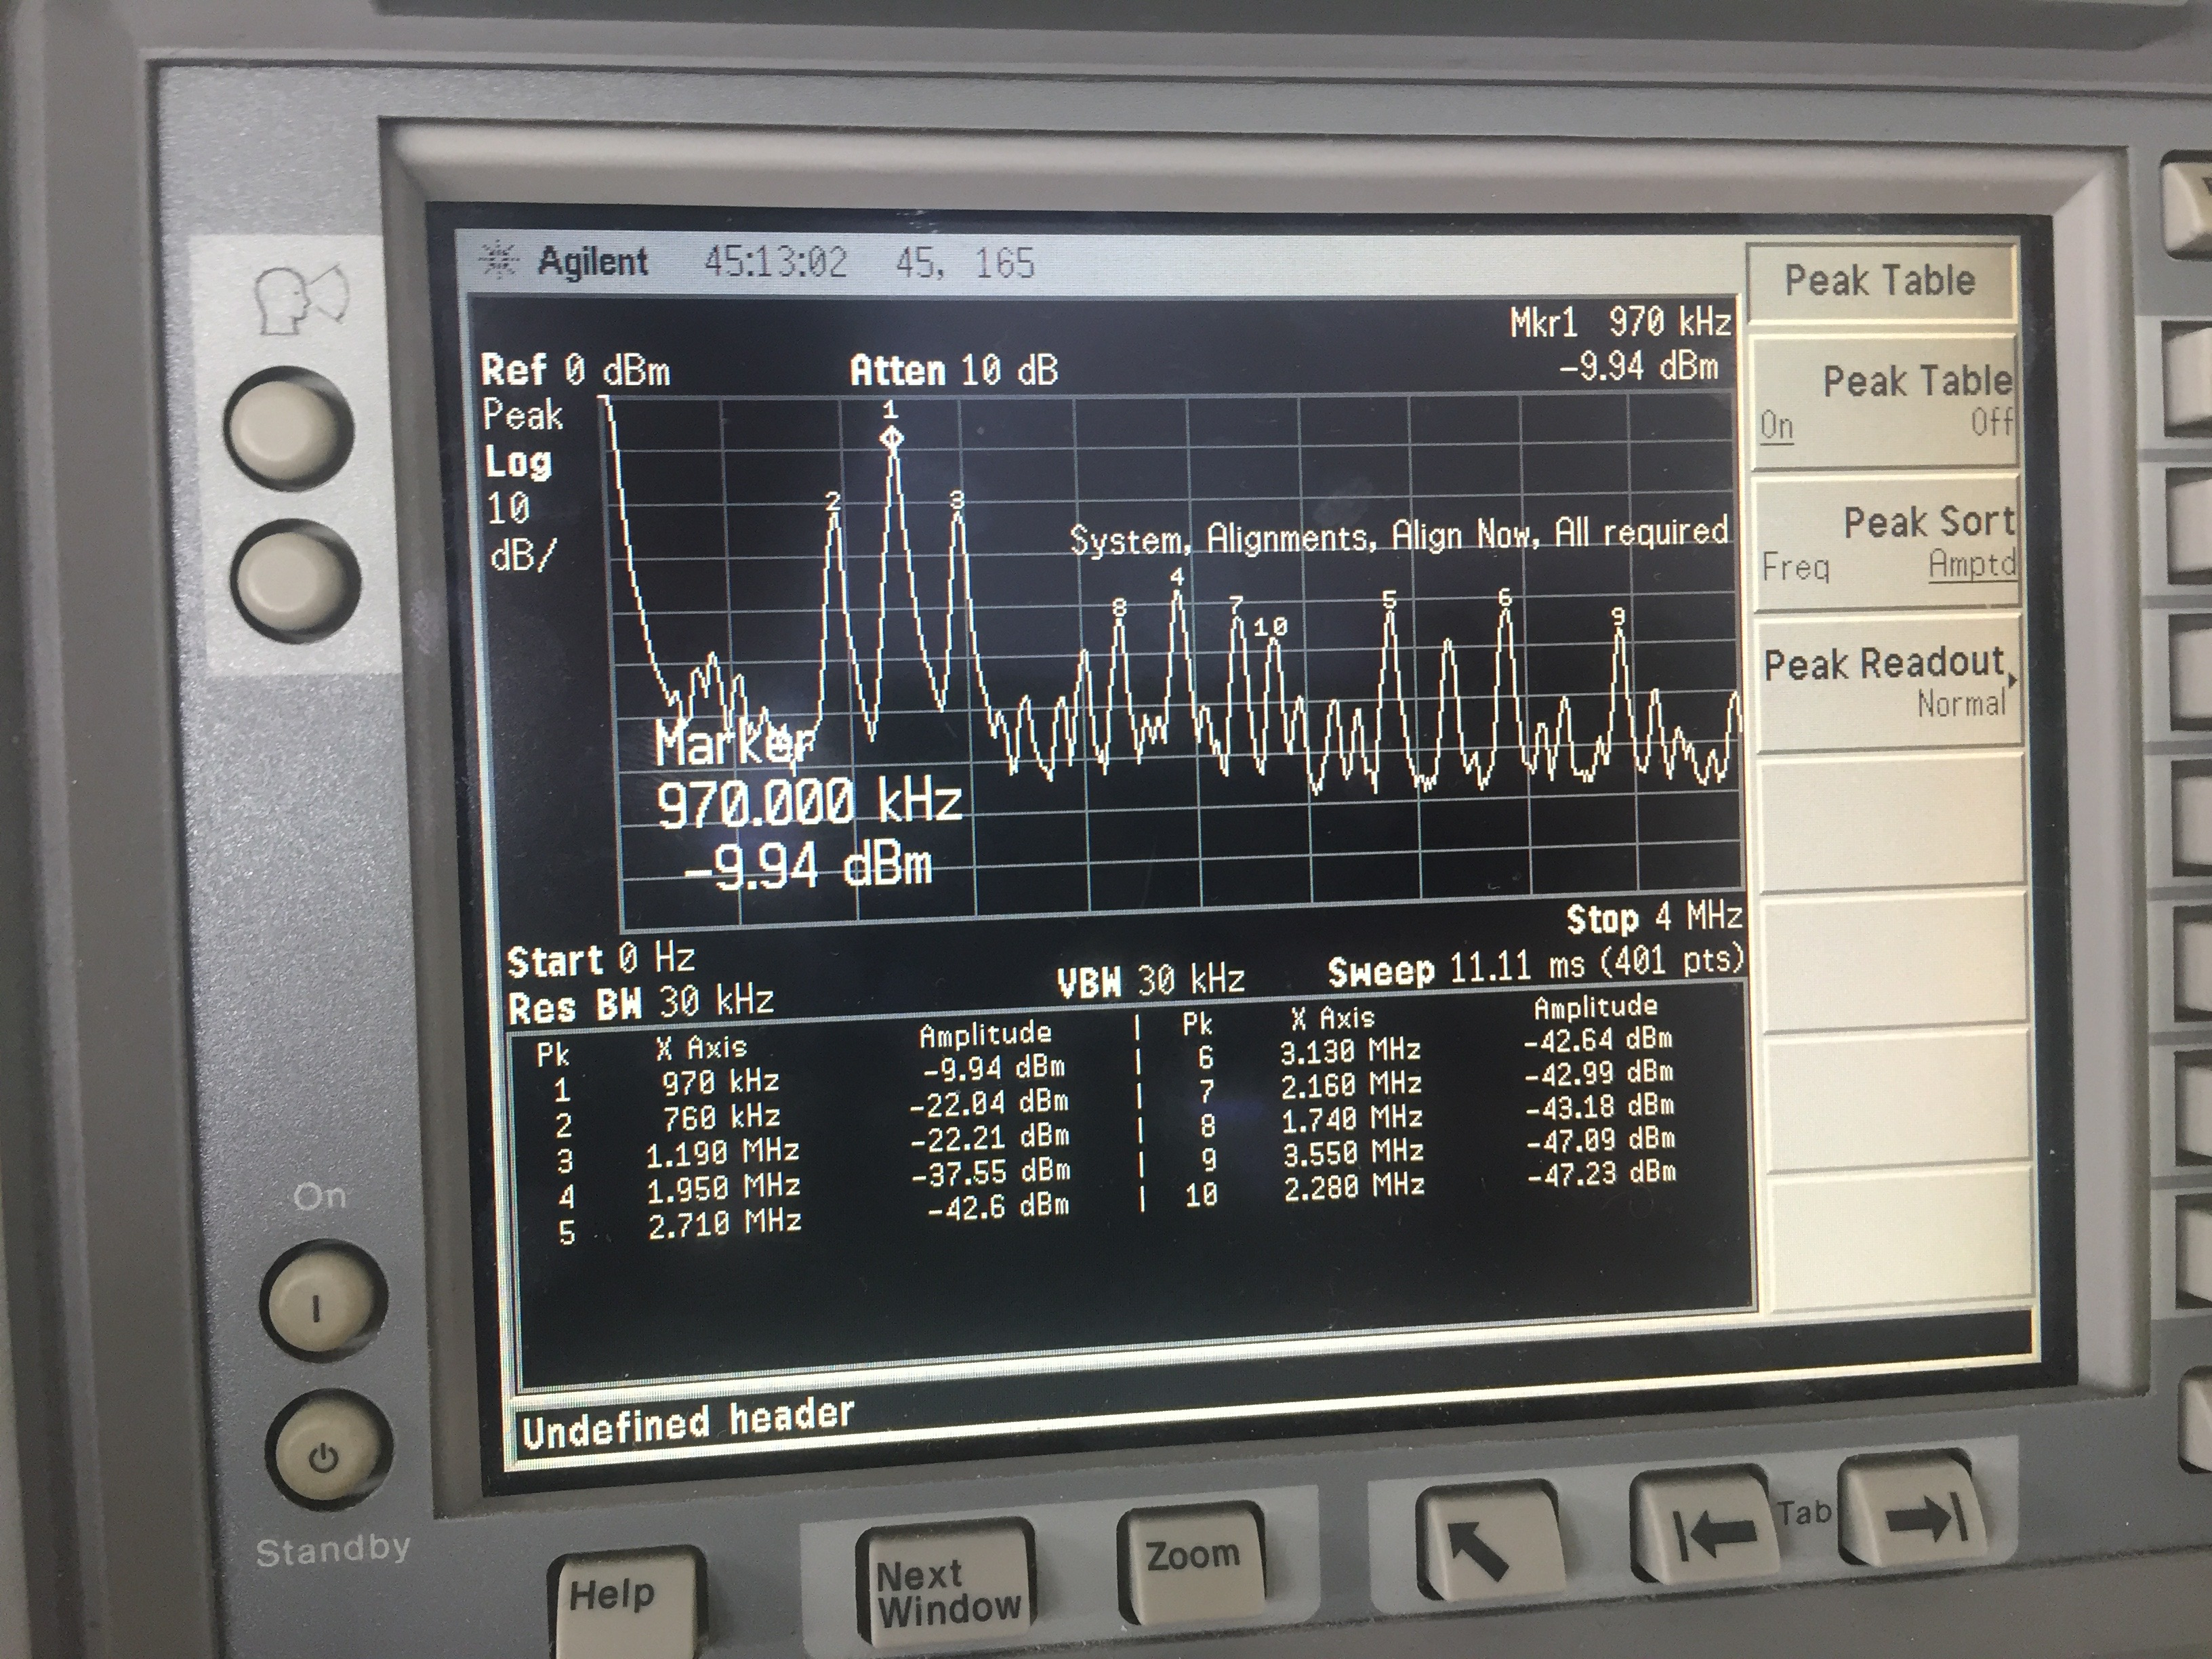
\includegraphics[width=.9\textwidth]{Spektrum_Pics/d.jpg}
  \caption{Frequenzspektrum der frequenzmodulierten Schwingung.}
  \label{fig:freqModSpek}
\end{figure}
Dort lassen sich für die Leistungspegel der drei höchsten Peaks die Werte mit entsprechenden Unsicherheiten ablesen:
\begin{align*}
  L_\text{P, links} &= \SI{-22.0(1)}{dBm} & L_\text{P, mitte} &= \SI{-9.9(1)}{dBm} & L_\text{P, rechts} &= \SI{-22.2(1)}{dBm}.
\end{align*}
Die Rechnung aus Kapitel \ref{sec:amplModDiode} wird nun hier mit den veränderten Amplituden für die beiden äußeren Peaks aus Gleichung \eqref{eqn:freqmod2} modifiziert. So ergibt sich für den Modulationsgrad hier:
\begin{align*}
  m &= \frac{2 U_\text{lr}}{U_\text{mitte}} \frac{f_\text{M}}{f_\text{T}}\\
  &= \num{0.1067(15)}.
\end{align*}
Damit kann die Forderung an die Schmalband-Frequenzmoduation überprüft werden. Mit
\begin{align*}
  m \frac{f_T}{f_M} = \num{0.491(7)} << 1
\end{align*}
ist diese erfüllt.

\subsection{Demodulation mithilfe eines Ringmodulators}

Mit der Schaltung aus Abbildung \ref{fig:expef} wird eine Messreihe von verschiedenen Frequenzen der Trägerspannung $f_\text{T}$ und der am Ausgang X anliegenden Gleichspannung $U$ aufgenommen.

Die beiden Spannungen, die an den Eingängen L und R anliegen, sind durch einen Phasenschieber mit einer Phasenverzögerung von $\Delta t = \SI{250}{\nano\second}$ zueinander verschoben.
Die Phasenverschiebung wird berechnet mit:
\begin{align}
  \Delta \phi = 2\pi \Delta t  f.
\end{align}
In Tabelle \ref{tab:phase} sind die aufgenommenen Werte sowie die berechneten Phasenverschiebungen zwischen den beiden Spannungen eingetragen.
In der Abbildung \ref{fig:plotphase} ist die Spannung gegen den Kosinus der Phase aufgetragen.
\begin{figure}
  \centering
  \includegraphics[width=.9\textwidth]{build/plotphase.pdf}
  \caption{Diagramm der Spannung in Abhängigkeit vom Kosinus der Phase. Die Unsicherheiten sind aufgrund ihrer geringen Größe nicht zu sehen.}
  \label{fig:plotphase}
\end{figure}
An die Messwerte wurde noch die Funktion
\begin{align}
  \cos(\Delta \phi) = m U + b
\end{align}
gefittet. Die bestimmten Fitparameter sind:
\begin{align*}
  m &= \SI{-6.4(2)}{\per\volt} & b &= \num{-0.01(3)}.
\end{align*}

Mit der Schaltung nach Abbildung \ref{fig:ampldemodschaltung1} wird eine amplitudenmodulierte Spannung demoduliert und auf dem Oszilloskop dargestellt. Das sich ergebende Bild ist in Abbildung \ref{fig:demodRing} zu sehen. Die demodulierte Spannung weist die ungefähr gleiche Frequenz auf wie die Modulationsspannung, allerdings ist ihre Amplitude deutlich kleiner.
\begin{figure}[h]
  \centering
  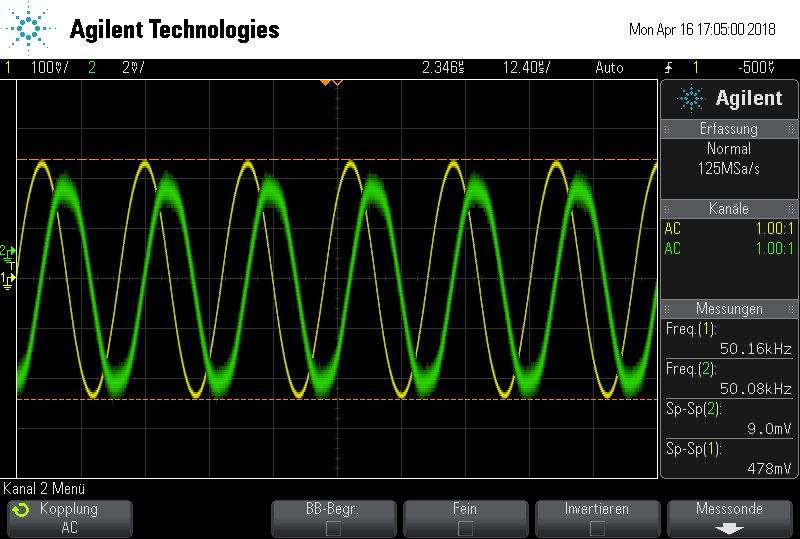
\includegraphics[width=.9\textwidth]{Oszi_Pics/demodRing.png}
  \caption{Oszilloskopbild der demodulierten Spannung(grün) sowie der Original-Modulationsspannung(gelb).}
  \label{fig:demodRing}
\end{figure}

\subsection{Demodulation mithilfe einer Gleichrichterdiode}

Nun wird mithilfe einer Gleichrichterdiode nach Schaltung aus Abbildung \ref{fig:ampldemodschaltung2} eine amplitudenmodulierte Spannung demoduliert.
Das aufgenommene Bild nach der Diode ist in Abbildung \ref{fig:gnachA} zu finden und das nach dem Tiefpass in Abbildung \ref{fig:gnachTiefpass}.
\begin{figure}[h]
  \centering
  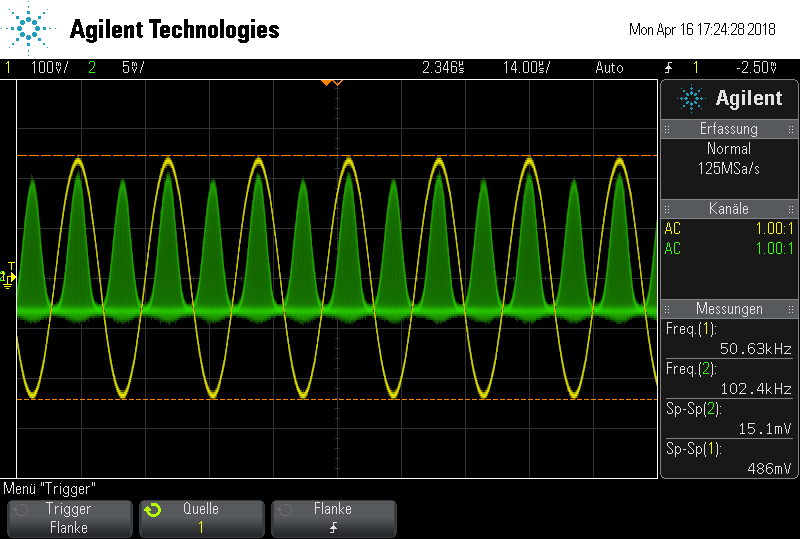
\includegraphics[width=.9\textwidth]{Oszi_Pics/gnachA.png}
  \caption{Oszilloskopbild der demodulierten Spannung(grün) sowie der Original-Modulationsspannung(gelb) nach der Diode.}
  \label{fig:gnachA}
\end{figure}
\begin{figure}[h]
  \centering
  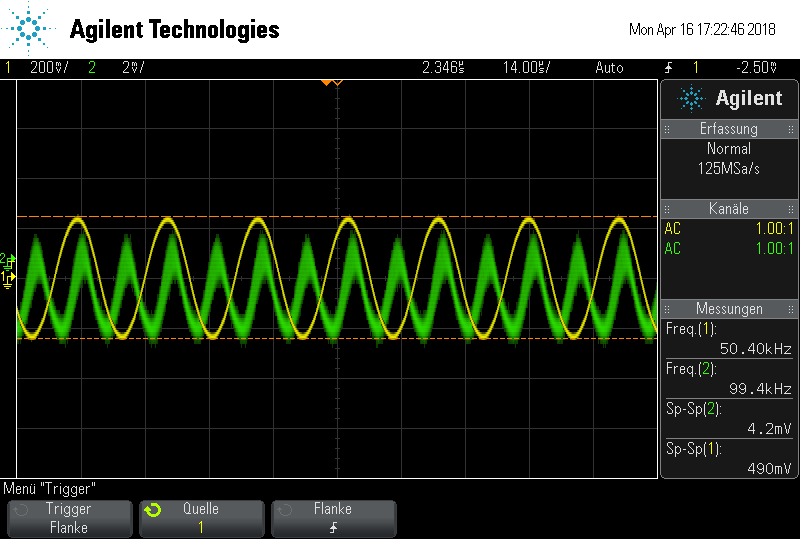
\includegraphics[width=.9\textwidth]{Oszi_Pics/gnachTiefpass.png}
  \caption{Oszilloskopbild der demodulierten Spannung(grün) sowie der Original-Modulationsspannung(gelb) nach dem Tiefpass.}
  \label{fig:gnachTiefpass}
\end{figure}
Zu erkennnen ist, dass die demodulierte Spannung die doppelte Frequenz der Original-Modulationsspannung hat. Die Amplitude der Spannung nimmt mit der Anzahl an dazwischengeschalteten Bauteilen ab.

\subsection{Demodulation einer frequenzmodulierten Spannung}

Zum Abschluss wird erneut eine frequenzmodulierte Spannung mit Abbildung \ref{fig:freqmodschaltung} erzeugt und mit der Schaltung nach Abbildung \ref{fig:flankendemodulator} demoduliert. Dann werden drei Bilder nach den verschiedenen Bauteilen aufgenommen.
Diese sind in den Abbildungen \ref{fig:hnachSchwingkreis}, \ref{fig:hnachDiode} und \ref{fig:hnachTiefpass} zu sehen.
Die Frequenz der Modulationsspannung ist in den jeweiligen Bildern auch in den Schwingungen nach den Bauteilen ablesbar. Nach dem Schwingkreis ist die Amplitude höher als die Ausgangsamplitude, wohingegen sie von den andern beiden Bauteilen reduziert wird.
\begin{figure}[h]
  \centering
  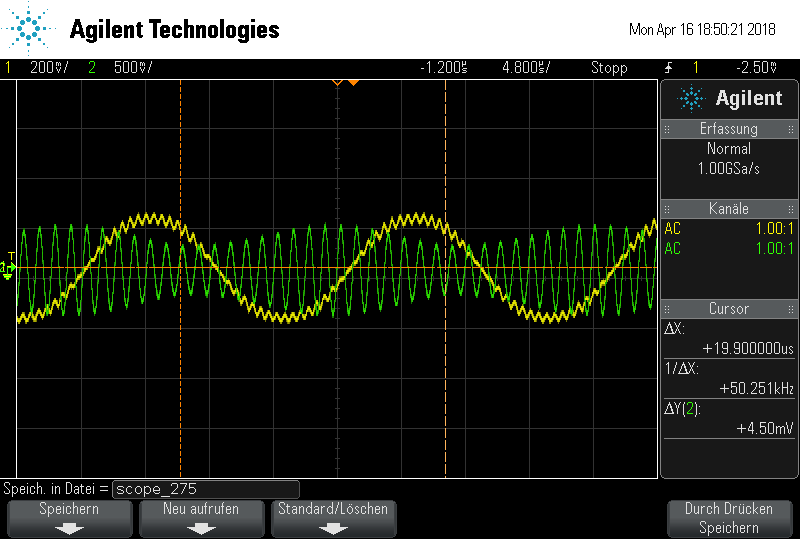
\includegraphics[width=.9\textwidth]{Oszi_Pics/hnachSchwingkreis.png}
  \caption{Oszilloskopbild der Spannung nach dem Schwingkreis(grün) mit der Modulationsspannung(gelb).}
  \label{fig:hnachSchwingkreis}
\end{figure}
\begin{figure}[h]
  \centering
  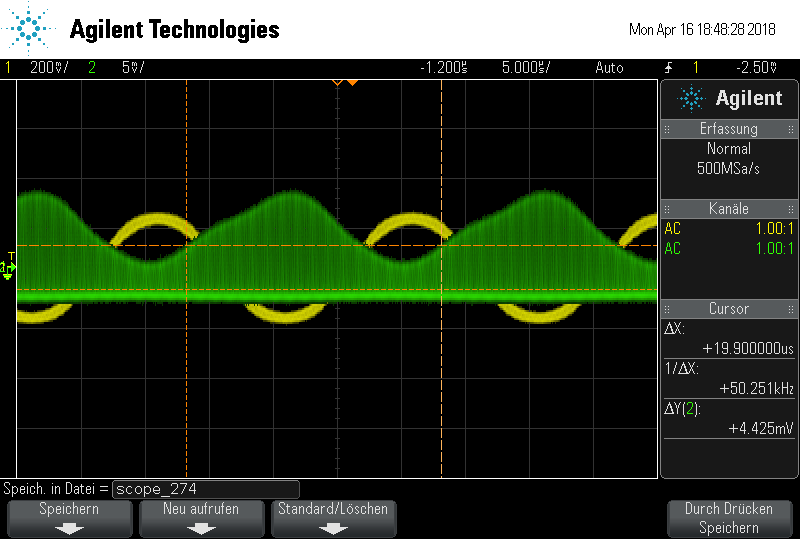
\includegraphics[width=.9\textwidth]{Oszi_Pics/hnachDiode?.png}
  \caption{Oszilloskopbild der Spannung nach der Diode(grün) mit der Modulationsspannung(gelb).}
  \label{fig:hnachDiode}
\end{figure}
\begin{figure}[h]
  \centering
  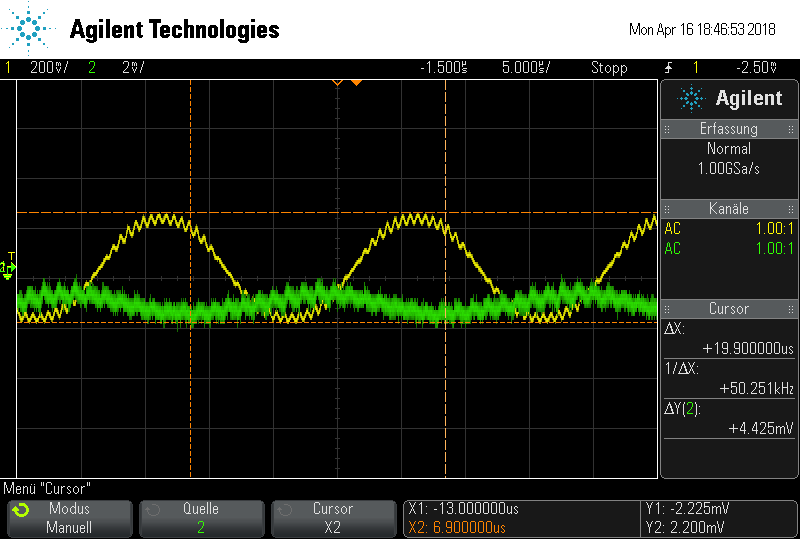
\includegraphics[width=.9\textwidth]{Oszi_Pics/hnachTiefpass.png}
  \caption{Oszilloskopbild der Spannung nach dem Tiefpass(grün) mit der Modulationsspannung(gelb).}
  \label{fig:hnachTiefpass}
\end{figure}
